
%
%  $Description: Author guidelines and sample document in LaTeX 2.09$ 
%
%  $Author: ienne $
%  $Date: 1995/09/15 15:20:59 $
%  $Revision: 1.4 $
%

\documentclass[times, 10pt,twocolumn]{article} 
\usepackage{latex8}
\usepackage{times}
\usepackage{graphicx}
\usepackage[font={it}]{caption}
\graphicspath{{Users/pedrolopes/Documents/PADI1314}}

%\documentstyle[times,art10,twocolumn,latex8]{article}

%------------------------------------------------------------------------- 
% take the % away on next line to produce the final camera-ready version 
\pagestyle{empty}

%------------------------------------------------------------------------- 
\begin{document}

\title{PADI-DSTM}



\maketitle
\thispagestyle{empty}


%------------------------------------------------------------------------- 
\Section{Introduction}
Since the beginning of the computer revolution in the world, the distributed systems have played a major role in the technologies' innovation and development. This area comprises a great set of different technologies and applications, like network applications, telecommunication networks, parallel computation, etc. In recent years we have been witnessing a new era in technology, the Cloud era. Today the Cloud is the new "big thing" in computers and mobile devices, everyone can access everything  everywhere! As such, the transactional shared memory systems are increasingly important in the world of technology, because nowadays the computers and mobile devices are using the cloud storage, and capacities, not only for save data but also for run programs, like the Amazon Silk, that is a web browser that processes the requests from the clients in the Amazon servers, and the client's devices only have to renderer the result data, to present the result. Due to this evolution of the distributed systems, the PADI-DSTM appeared.This library intends to implement a distributed system to manage objects stored in a distributed shared memory, that are shared by transactional applications that are being executed in different machines. This library intends to provide an easy way for the programmers doesn't have to deal with the distributed systems and transactions problems, like deadlocks, inconsistent data or data that disappears because a server fails, etc. The programmers only have to integrate the PADI-DSTM in his application, and the management of the transactional shared memory is all made by the library.

%------------------------------------------------------------------------- 
\Section{Architecture Overview}
%DONE RENATO

This work focuses on implementing a transactional shared memory system, which stores variables of PADInt type. These variables will be shared between the multiple clients of the system and will be located in a set of transactional servers, that replicate information in case of failure occurrence. Clients, recurring to the PADI-DSTM library, create and access variables on the system recurring to a master server, which maintains information about, and manages the location of each one of them. Once accessed, clients can execute transactions, that encapsulate read and write operations on a subset of these variables, preserving the Atomicity, Consistency, Isolation and Durability (ACID) properties. One of the main concerns of this work is trying to implement the system in a decentralized way, minimizing the interaction with centralized entities. For doing so, it considers client as the transaction coordinator, in contrast with master, once it is assumed clients never crash. The interactions with the master server will be only for creating and accessing data objects. The system will consider a fault model which tolerates one silent failure. For doing so, it implements an active replication protocol with 3 replicas, and a quorum of 2 servers. The system will follow a two-phase commit protocol for executing the transactions, which, as mentioned before, will take as coordinator the transaction client, and as participants the servers which hold the involved data objects. Finally, the master server will be able to mediate the load between transactional servers, reallocating resources in order to preserve the equal distribution of network and storage loads, which favors the systems scalability. The next sections will expose the systems behavior with more detail.



%------------------------------------------------------------------------- 
\SubSection{Data Structures}

Our PADI-DSTM library contains multiple data structures with different goals. In the Master server are stored the list of transactions unique identifiers that started and ended, in order to have a log of the transactions that have been completed, and if one transaction id only exists in the list of started transactions, this means that the transaction has been aborted. The servers continually send  heartbeats messages("I'm alive") to the Master which updates a list that contains the active servers, and when the client connects with the Master by calling the methods AccessPadInt or CreatePadInt, the Master only returns the active servers in the object that contains the PadInt. In heartbeats messages the servers also include the number of active connections at the time, in order to the master know which servers have a greater number of connections and when a client requests the servers to the master, the master only returns the ones with less number of connections.  

The PadInt object is the main one in our architecture, it is stored in the servers, and each PadInt exists in three servers, in order to tolerate faults. Each of the three objects is always updated to the last version, because when the changes to the object are committed, the new values are propagated to the other servers in which the object is stored. The PadInt object contains different sub-objects, its UID (to make each PadInt unique), its value, an array of the servers in which it is stored (we decided that each object know its own location, and the client decides which one to bind to, when he receives the object through the API). The PadInt object also contains a timestamp that it is used to control the accesses to the variable in the memory, in this case if the client timestamp is lower than the timestamp of the object it means that the client has an old version of the object and the transaction is aborted.

\begin{figure}[h!]
	\centering
	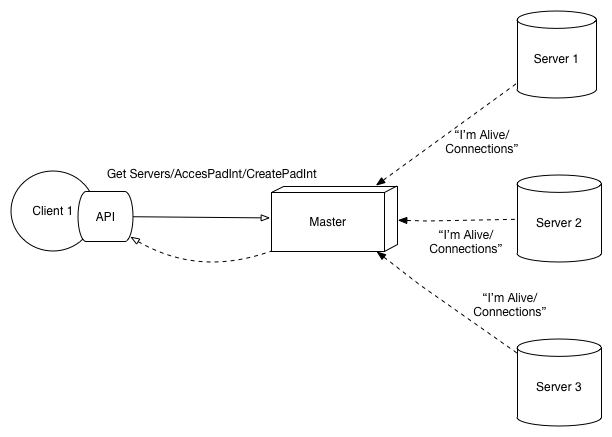
\includegraphics[scale=0.4]{Client-Master.png}
	\caption{Diagram to show client requests to master and servers heartbeat messages to  master}
\end{figure}

%------------------------------------------------------------------------- 
\SubSection{Responsibilities}

As seen before, our approach will be divided in three components, a master, a client and a transactional server, each one of them with distinct roles.
The master, has three main responsibilities. The first one is to store meta-data regarding transactional servers and data objects existing in PADI-DSTM. It stores among other information, object location and uid, or transactional servers location and network load. The second role of master server is to mediate the creation and access to shared variables. Clients connect to the master for getting remote objects that represent variables. In case of a creation, the master will choose the most unloaded transactional servers and  execute a create operation. Master is also the one who executes the load balancing algorithm, for coordinating and re-allocating resources. Basing on a timer, the master server will execute a load balancing algorithm, which distributes work equally amongst the servers.
The second one, the transactional servers will store and execute the changes made to the data objects, acting as participants of a distributed transaction protocol. They are responsible for managing the variable locks, committing or aborting transactions depending on the conditions they have for maintaining the ACID properties of each transaction. They also indicate the master their activity through a heartbeat message, which carries the number of active connections, informing the master of their current network load.  
Finally, clients will execute the programs that use the PADI-DSTM library, invoking the creation/access to the objects on the master and manipulating them on the transactional servers. Clients will also, through the PADI-DSTM library, act as coordinators for the transactions they trigger. Clients connect to the servers that are currently storing the variables they want to modify and trigger a two-phase commit protocol.

\begin{figure}[h!]
	\centering
	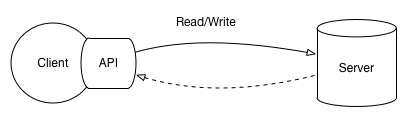
\includegraphics[scale=0.45]{Client-Server.png}
	\caption{Client-Server connections}
\end{figure}

%------------------------------------------------------------------------ 
\SubSection{Concurrency Control}
With a distributed system, there's a problem that is inherent to this type of architecture: concurrent access to shared objects. In this particular case, we have to take into consideration that objects can be accessed by multiple clients and, when committing the changes, the objects may be accessed by several servers as well.
To manage this type of concurrency, we will be using timestamp-based concurrency control. This type of approach assigns a timestamp (which can be a time value or a sequence number) to the transactions that want to have access over a certain object. This object also keeps a timestamp of its own and also keeps track of the latest transaction that read/wrote the object's value. With this kind of approach, the transactions are forced, in a sense, to access the object in a specific order, so that there are no actual parallel accesses.
One aspect that is important to mention is that there is still a lock on the object that is being accessed, though this is not a "fully grown" lock as it would be in database lock-based concurrency control. The lock is to prevent concurrent access to an object, though the time the lock is locked is significantly smaller and there is no chance of deadlocking since the lock is immediately released when it's no longer needed, as opposed to lock-based concurrency control in which the locks are released at the end of the transaction.

%------------------------------------------------------------------------- 
\SubSection{Transactional Algorithms}


For guaranteeing the conformity with ACID properties, our solution will implement a transaction protocol between the servers involved in an operation. It implements a slight variation of a Two-phase commit protocol(2PC), where the client plays the role of coordinator, and the transactional servers act as participants. Taking the client machine as the transaction coordinator is possible since we can assume (i) the clients don't crash, (ii) client and transactional servers are the only ones who are involved in a given transaction. This way our solution avoids the bottleneck of centralizing the coordination on the master server. On the other hand, if the coordination task was given to another unrelated transactional server, it could lead to protocol deadlocks, since it is assumed transactional servers can crash.
The protocol initiates calling beginTx() operation, which launches a coordination object in the client, through the PADI-DSTM library. This object has an endpoint with a given address, and creates a transaction identifier (tid). Each operation executed on each of transactional server will carry the tid and address of coordination endpoint so that they join the current transaction. Once all servers are joined, the protocol carries out through the following two phases.
\begin{itemize}

\item[--] Phase one: Voting

\begin{enumerate}
	
\item The coordinator send a \emph{prepare} message to each participant.

\item Basing on the operation viability, each participant replies \emph{yes} or \emph{no} to the prepare request. In affirmative case, it prepares to commit saves objects into partition storage. In case of a negative answer, it has to completely abort the transaction.

\end{enumerate}

\item[--] Phase two: Deciding

\begin{enumerate}

\item The coordinator decides whether the transaction commits or aborts basing on the votes returned from participants. If all the participants vote to commit, and no failure has occurred, the coordinator decides to commit the transaction and sends a \emph{doCommit} request to every participant. In case of any participant vote to abort, the coordinator signals all the participants to abort the transaction. 

\item The participants receive a response from coordinator and do whatever it prescribes them to do (commit or abort). In case of a \emph{doCommit} participant returns a \emph{haveCommited} call to inform the coordinator that the transaction is finished. In case of abort, they simply abort the transaction.


\end{enumerate}

\end{itemize}

Once its assumed that transactional servers can crash and the network can delay the delivery of messages, the protocol peers (coordinator and participants) are required to limit the time they wait for a response. Therefore, the protocol implements a series of timeout procedures in order to avoid situations where the peers wait indefinitely. 
Firstly, consider the situation where the participant voted \emph{yes} and is waiting for a decision from the coordinator. Since this is assumed as not crashing, the only reason the participant can wait a long period of time is due to a network delay. For resolving this issue, the participant, in presence of a similar situation, must inquiry the coordinator for a decision (through a \emph{getDecision} call). The coordinator then replies and the participant gets its decision.
The second situation related to the phase where the coordinator waits for the votes from all the participants. If one or more of these servers crash or gets a network delay, the coordinator must not wait indefinitely. In this case, it counts down a timer. Once it reaches timeout, the coordinator sends \emph{doAbort} messages to all the transaction participants.

\begin{figure}[h!]
	\centering
	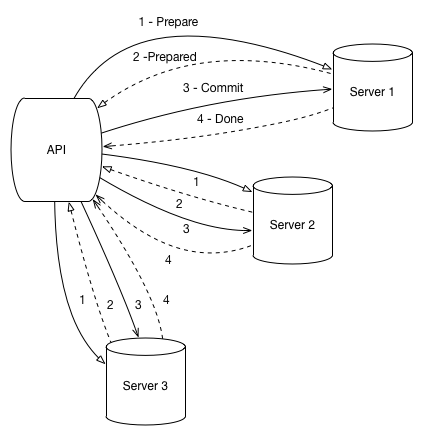
\includegraphics[scale=0.45]{2PC.png}
	\caption{Our two-phase commit aproach}
\end{figure}

%Porque o client?
%protocolo
%timeouts


%------------------------------------------------------------------------- 
\SubSection{Distributed Protocols}

As indicated above, our aproach will take into account the problem of overloading servers, in this case, the problem is that, at certain point in time, it is possible that some servers will be more loaded than others, or if new servers are connected to the master, that servers will be empty, and the others can be full, and because they have all the objects, the requests will be always made to the loaded servers, while the new servers stay empty. To resolve the problem our solution will be divided in three parts, the first part is that the master will have a registry of the location of the objects, so the master can always see which servers are more loaded. the second part of the solution is thar the master, as indicated above, will receive heartbeat messages, and those messages the servers will indicate the master that they are still active, and the number of connections at the time, with that information the master will upate his registry of the active servers and connections of that servers, and when a new client requets the server to some object the master will try to give him the less loaded server  with less number of connections, if possible. And the third part of the solution is that our master server will have a timer, that from time to time activates a trigger will, and when that happens, a special type of transaction will be occurr. In that special transaction the master will see, in his list of servers and locations, which servers are more loaded, and transfer part of the data to servers that are less loaded, after tranfering the data, the master will update the location of the objects in his registries, so that when a client request the access to some PadInt he always receives the new location, and not the reference to the object previous location.  

%TODO: DELTAS

%------------------------------------------------------------------------- 
\SubSection{Deadlock Detection and Abort Recovery}
Bearing in mind that we're using timestamps to prevent concurrent access to shared objects, the greatest advantage when using this type of concurrency control is that there are no deadlock situations, since the access to shared objects aren't locked by another data type, like the locks used in database transactions or the OS's mutexes.
Even though this concurrency control method avoids deadlock through its implementation, there are some situations where the occurring transactions abort without a conflict of two (or more) of those transactions accessing the same shared object. This sort of thing happens when, for example, a transaction T1 has a timestamp value of 100 and another transaction T2 has a timestamp value of 200. If T2 tries to read an object (without altering its value) before T1, though there are no read-write/write-write/write-read conflicts, both T1 and T2 must abort because the access to the object wasn't sequential (since T1 has a lower timestamp value than T2).
To overcome what was stated above, we will take into account what actions the transactions want to execute. By doing so, if two transaction only read the value from an object without altering it, even if they perform these actions inconsistently with the assigned timestamps, there is no need to abort because the operations' outcome will never generate an inconsistency, as long as there aren't any modifications to the object's value.

\Section{Conclusions}

In this article we present a solution for PADI-DSTM. With the adopted aproaches to the problem we belive that our solution will not have much problems in terms of scalability, because connect new servers to master is very easy to be done, the load balance solution will try to ensure the load equality between servers. Our load balance sloution helps to control the number of connections clients-servers, because the master is the one who controls which servers the client receives to try to bind.

Our solution gives particular emphasis to the Two-phase commit protocol to control the ACID problems of transactions, and because our transaction coordinator is the client, the master it isn't a bottleneck in the system. Other solutions coul be adopted, like servers comunicate between each other in the commit phase to store the data, this could make our transactions faster, because the 2PC is a slow algorithm, but this solution will bring us other sort of problems, like the main server fail during the commit phase.

Finally, we believe that our solution can be be improved, and we expect to do so in the near future.

%------------------------------------------------------------------------- 

\bibliographystyle{latex8}
\bibliography{latex8}

\begin{thebibliography}{9}
 
\bibitem{Distributed Systems, Concepts and Design}
George Coulouris, Jean Dollimore, Tim Kindberg, Gordon Blair,
   Distributed Systems, Concepts and Design, 
   Pearson,
   5th edition,
   2012.

\end{thebibliography}

\end{document}

